\documentclass[conference]{IEEEtran}
\IEEEoverridecommandlockouts
\usepackage{cite}
\usepackage{amsmath,amssymb,amsfonts}
\usepackage{algorithm}
\usepackage{algpseudocode}
\usepackage{graphicx}
\usepackage{textcomp}
\usepackage{xcolor}
\usepackage{booktabs}
\usepackage[caption=false,font=footnotesize]{subfig}
\def\BibTeX{{\rm B\kern-.05em{\sc i\kern-.025em b}\kern-.08em
    T\kern-.1667em\lower.7ex\hbox{E}\kern-.125em X}}
\renewcommand{\algorithmicrequire}{\textbf{Input:}}
\renewcommand{\algorithmicensure}{\textbf{Output:}}
\algrenewcommand\algorithmicindent{0.9em}

\begin{document}

\title{Explainable Resume and Job Matching with\\Hybrid Features and Weak Supervision}

\author{
\IEEEauthorblockN{1\textsuperscript{st} Shivani Srivastava}
\IEEEauthorblockA{\textit{School of Computer Science and Engineering (SCOPE)} \\
\textit{Vellore Institute of Technology}\\
Vellore, India \\
shivani.srivastava2023@vitstudent.ac.in}
\and
\IEEEauthorblockN{2\textsuperscript{nd} Megana Subash}
\IEEEauthorblockA{\textit{School of Computer Science and Engineering (SCOPE)} \\
\textit{Vellore Institute of Technology}\\
Vellore, India \\
megana.subash2023@vitstudent.ac.in}
}

\maketitle

\begin{abstract}
Screening a resume against a vacancy needs word-level and meaning-level comparison, and a reviewer must be able to see why a candidate received a given score. Public resume collections carry occupation labels but no job descriptions and no relevance judgments, which are exactly what supervised matching requires. This paper presents a pipeline that merges term-frequency features, pretrained sentence embeddings and structured profile attributes for explainable resume and job analysis. A calibrated linear support vector machine predicts the occupational category. A gradient-boosted classifier with isotonic calibration scores each resume and job pair from 17 features, a separate LambdaRank model orders candidates, and TreeSHAP reports feature contributions. Experiments use 2,481 processed resumes from 24 categories, together with synthetic job descriptions and relevance grades derived from categories. The role classifier reaches 71.43 percent accuracy and a macro-F1 of 0.6716 on 497 test resumes. On 11,520 held-out pairs the calibrated classifier attains a ROC-AUC of 0.8041, against 0.7692 for TF-IDF cosine similarity, and calibration lowers the expected calibration error from 0.0233 to 0.0177 while the Brier score is unchanged. Ablation results suggest that lexical, semantic and structured signals complement one another. Three problems restrict the conclusions: a false-negative rate of 50.44 percent, sensitivity to identity text, and ranking metrics that depend on tie handling. The contribution is an inspectable hybrid prototype and a critical review of its weak-supervision benchmark, which states what real job descriptions and independent relevance judgments would be needed to validate it.
\end{abstract}

\begin{IEEEkeywords}
resume analysis, semantic matching, weak supervision, LightGBM, learning to rank, model calibration, explainable machine learning
\end{IEEEkeywords}

\section{Introduction}
Matching a resume to a job description is at once a text-understanding problem and a decision-support problem. Evidence about an applicant is spread across work history, skills and qualifications, whereas a vacancy states its needs in different wording. Plain term overlap is easy to compute but overlooks related phrasing, and a broad occupational label cannot show whether one particular requirement is satisfied. A practical system therefore has to treat these questions separately and give the human reviewer enough evidence to verify its output.

Term frequency--inverse document frequency (TF-IDF) is an efficient lexical representation \cite{b1}, and sentence embeddings make it possible to compare texts that share little vocabulary \cite{b2}. Neither encodes an experience shortfall, an education level or a missing skill explicitly. Adding structured attributes is a sensible engineering step, yet a learned score only has meaning relative to the supervision behind it. If relevance labels come from occupational categories, the model learns that proxy relation rather than independently established suitability for hiring.

This work examines a hybrid pipeline under precisely that restriction. A role classifier runs separately from a resume--job feature model, and the latter yields calibrated compatibility estimates, a candidate ordering and feature-level explanations. The evaluation covers discrimination, calibration, ranking, ablation and sensitivity to identity text. The guiding question is whether structured and semantic features contribute beyond lexical evidence on the available benchmark, and which properties of the evaluation restrict that conclusion.

The contributions are listed below.
\begin{enumerate}
\item A fixed 17-feature representation that fuses lexical, semantic and structured signals and is shared by training and inference.
\item An explainable application that returns role classification, calibrated compatibility, learned ranking and attribution as four distinct outputs.
\item A controlled weak-supervision benchmark built from category-labelled resumes, with graded relevance and splits that are disjoint at the job and record level.
\item A critical analysis of the recorded experiments, covering calibration trade-offs, label validity, false negatives, identity sensitivity and the effect of ties on ranking metrics.
\end{enumerate}
No new encoder architecture is proposed, and no claim is made of outperforming commercial recruitment products.

The remainder of the paper is organized as follows. Section~II reviews related work, Section~III formalizes the problem, Section~IV describes the method, Section~V presents the system, Section~VI details the experimental setup, Section~VII reports results, Section~VIII discusses limitations, and Section~IX concludes.

\section{Related Work}
\subsection{Lexical and Semantic Representations}
Vector-space retrieval weights informative terms and compares document vectors cheaply, but it depends on the vocabulary actually seen \cite{b1}. Sentence-BERT applies siamese and triplet networks to produce sentence embeddings that can be computed once and reused, so pairs need not be scored jointly \cite{b2}. This suits comparing many resumes against a single vacancy, although one pooled vector can conceal which passage backs an individual requirement. MiniLM compresses pretrained Transformers through self-attention distillation \cite{b3}; it supplies the compact semantic component used here and is not specific to recruitment.

\subsection{Boosted Trees and Learning to Rank}
LightGBM provides gradient-boosted trees that combine heterogeneous inputs and model nonlinear interactions \cite{b4}, which helps when similarity and qualification evidence must be weighed together. Our implementation calls its classifier and ranker interfaces and does not assert that every optimization of the original paper is active. Burges distinguishes ranking-oriented learning from ordinary classification through RankNet, LambdaRank and LambdaMART \cite{b5}; following that distinction, shortlist order and probability estimation are handled here as separate outputs. Ranking quality is measured with normalized discounted cumulative gain (NDCG) \cite{b6}.

\subsection{Explanation and Calibration}
SHapley Additive exPlanations (SHAP) assign additive contributions to single predictions \cite{b7}, and TreeSHAP computes them exactly for tree ensembles \cite{b8}. An attribution shows how a model combines numerical evidence; it can neither validate the target labels nor establish causality. Calibration relates predicted scores to observed label frequencies. Isotonic regression is a nonparametric monotonic mapping \cite{b9}, and expected calibration error (ECE) is a common summary of miscalibration \cite{b10}.

\subsection{Weak Supervision and Fairness in Hiring}
Weak supervision trains models on programmatically generated labels in place of manual annotation \cite{b11}. It allows learning when ground truth is absent, but the resulting scores measure agreement with the labelling rule. Audit studies of name-based discrimination \cite{b12} and reviews of algorithmic hiring \cite{b13} give reason to test whether identity text alters model outputs even when no protected attribute is an explicit input. These strands motivate an integrated and inspectable design, but none of them establishes real-world recruitment validity, which depends on the data, the labels and the evaluation design.

\section{Problem Formulation and Research Gap}
\subsection{Research Gap}
At the project level, the gap is the absence of one workflow that links structured extraction, occupation prediction, learned job compatibility, ranking and explanation. A keyword score ignores semantic relations, an embedding score lacks explicit qualification features, and a category label is too coarse to describe a specific vacancy. The available data also contain no genuine job descriptions or pairwise relevance judgments, so candidate suitability cannot be validated directly.

\subsection{Problem Definition}
Let $R$ be a text resume and $J$ a job description. The system produces four outputs, kept apart deliberately.
\begin{enumerate}
\item Role distribution: $\hat{c}(R)\in\Delta^{23}$, a probability vector over the 24 occupational categories.
\item Compatibility: $\hat{p}(R,J)\approx P(y=1\mid \mathbf{x}(R,J))$, where $\mathbf{x}\in\mathbb{R}^{17}$ is the pair feature vector and $y=\mathbf{1}[\mathrm{rel}(R,J)\ge 2]$ is the weak label defined in Section~IV.
\item Ordering: for a pool $\{R_i\}_{i=1}^{n}$ with $2\le n\le 30$, a permutation $\pi_J$ that sorts candidates by a learned ranking score $s_i$.
\item Explanation: per-feature contributions $\phi_k(R,J)$ for the compatibility classifier.
\end{enumerate}
Keeping the outputs apart prevents a category confidence from being read as a job-match probability, and a rank position from being read as a calibrated likelihood.

\section{Methodology}
\subsection{Corpus Preparation and Structured Extraction}
The source data are Bhawal's Resume Dataset \cite{b14}. The training scripts discard records lacking text or category, remove exact duplicates of the raw text and keep documents longer than 50 cleaned characters. The processed corpus holds 2,481 resumes in 24 categories. A stratified 80/20 split with seed 42 gives 1,984 training and 497 test records. Splitting is by record, and exact-text deduplication cannot show that differently worded records come from different real people.

PDF, DOCX and TXT inputs are converted to plain text. The raw text is retained for education and date parsing, while the model text is lowercased, stripped of URLs and email-like strings, limited to English letters plus ``+'' and ``\#'', and whitespace-normalized. Skill mining collects recurring one- to three-word phrases from recognized skills sections (a 1,800-character window, with stop-word, blacklist and document-frequency filters) and adds seed skills and aliases, which yields 419 canonical entries; inference applies longest non-overlapping matching. Education is the highest detected level on a scale from zero to four. Resume experience is the larger of the stated years and the combined length of recognized year intervals, capped at 45 years, whereas the job parser takes the first recognized years expression. These estimates do not verify employment or credentials. Required, preferred and title-derived skills are merged into one job-skill set, so ``required-skill coverage'' in fact measures coverage of all parsed job skills.

\subsection{Lexical and Semantic Representations}
The TF-IDF vectorizers use unigrams and bigrams, English stop words, sublinear term frequency, a minimum document frequency of two, a maximum document-frequency fraction of 0.9 and at most 30,000 features. Role classification and pair matching rely on separately fitted vectorizers. With the default L2 normalization, the dot product of two vectors equals their cosine similarity.

Semantic vectors come from the pretrained all-MiniLM-L6-v2 checkpoint, which outputs 384-dimensional embeddings \cite{b15}. A document is divided into 180-word chunks and at most four are retained, so no more than 720 cleaned words contribute. Writing $e(c_i)$ for the normalized embedding of chunk $c_i$, the document vector is
\begin{equation}
v(d)=\frac{\sum_{i=1}^{q} e(c_i)}{\max\left(\left\|\sum_{i=1}^{q} e(c_i)\right\|_2,\ \epsilon\right)},\quad q\le 4,
\end{equation}
with $\epsilon=10^{-9}$; its direction equals that of the normalized average. The embedding similarity is $s_{\mathrm{emb}}=v(R)^{\top}v(J)$. The encoder's default 256-wordpiece limit may truncate a chunk further, and no task-specific fine-tuning is applied.

\subsection{Synthetic Jobs and Weak Relevance Labels}
Category statistics are computed from training resumes only. Skills are ranked by a frequency-weighted log-ratio of category frequency to corpus frequency, up to 40 per category are retained, and alternating entries form the principal training and test skill pools. Three templates combine titles, sampled skills, experience derived from category quantiles (scaled to between one and ten years) and the modal education level. This produces 720 training and 288 test descriptions. Algorithm~1 summarizes the construction and Fig.~1 shows the resulting data flow.

\begin{figure}[!t]
\centering
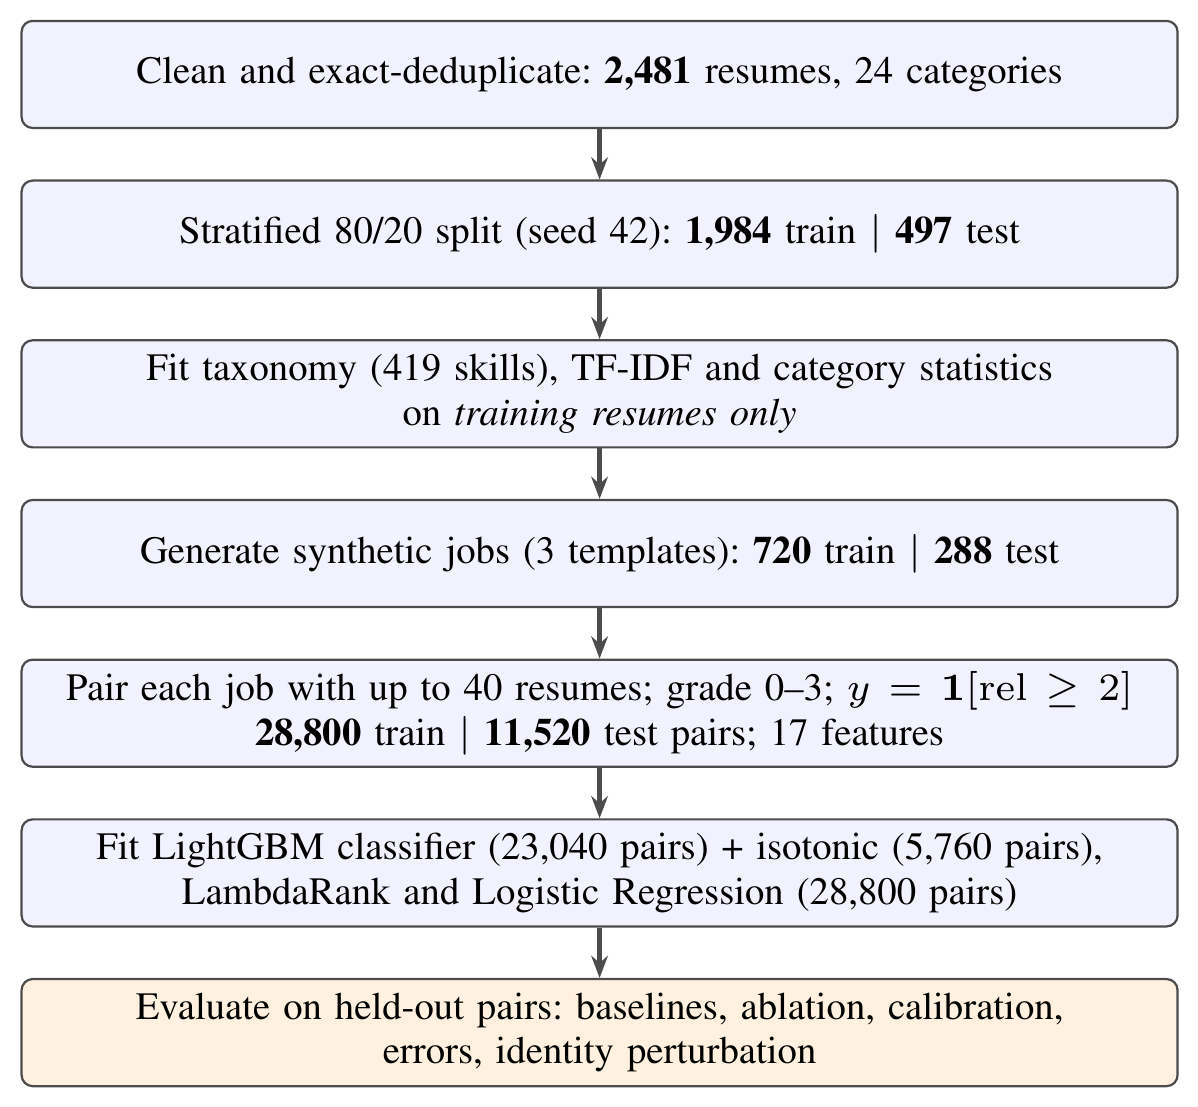
\includegraphics[width=0.82\columnwidth]{figs/fig1.png}
\caption{Benchmark construction and training/evaluation workflow. Counts are taken from the recorded experiment artifacts.}
\label{fig:workflow}
\end{figure}

\begin{algorithm}[!tb]
\caption{Weak-label benchmark construction (per split)}
\small
\begin{algorithmic}[1]
\Require resume records $D$ with categories; close-category sets $N(c)$; broad families $F(c)$
\Ensure job set $\mathcal{J}$ and graded pairs $\{(r,j,\mathrm{rel},y)\}$
\For{each category $c$}
  \State rank skills by frequency-weighted log-ratio; keep top 40; assign alternating entries to the split's principal pool $S_c$
\EndFor
\For{each job $j$ with target category $c_j$}
  \State sample a title, 4--6 required skills from $S_{c_j}$ and preferred skills (with probability 0.15, one from an unsplit pool of another category)
  \State set experience from category quantiles and education to the modal level; render with one of three templates
  \State draw $\le 10$ same-category, $\le 10$ related-category and the remaining other-category resumes (up to 40)
  \For{each candidate $r$ with category $c_r$}
    \State $\mathrm{rel}\leftarrow 3$ if $c_r=c_j$; $2$ if $c_r\in N(c_j)$; $1$ if $F(c_r)=F(c_j)$; else $0$
    \State $y\leftarrow \mathbf{1}[\mathrm{rel}\ge 2]$
  \EndFor
\EndFor
\end{algorithmic}
\end{algorithm}

Relevance is 3 for identical categories, 2 for explicitly listed close categories, 1 for a shared broad family (technology, business, creative or service) and 0 otherwise. The binary compatibility label is $y=\mathbf{1}[\mathrm{rel}\ge 2]$. The benchmark holds 28,800 training and 11,520 test pairs. Test grades 0 to 3 occur 5,868, 2,119, 761 and 2,772 times, so 3,533 pairs (30.7\%) are positive.

Candidate records and generated jobs are separated between training and test, but the separation is partial. A preferred skill may come from an unsplit pool, the fallback generator can reuse a complete pool, and templates, title sources and category statistics are shared. The benchmark therefore measures transfer to held-out records and generated descriptions rather than to independently collected vacancies. Education and experience mismatches do not alter the category-derived labels.

\begin{table}[!t]
\caption{Implemented Resume--Job Feature Groups}
\label{tab:features}
\centering
\small
\begin{tabular}{@{}llp{4.7cm}@{}}
\toprule
Group & \# & Features \\
\midrule
Semantic/lexical & 2 & embedding cosine; TF-IDF cosine \\
Skills & 6 & coverage, matched count, missing count, Jaccard, job-skill count, resume-skill count \\
Experience & 5 & resume years, job years, capped ratio, gap, meets requirement \\
Education & 4 & resume level, job level, gap, meets requirement \\
\bottomrule
\end{tabular}
\end{table}

\subsection{Pair Features}
Table~\ref{tab:features} lists the 17 implemented features. Early project documents mention 18, but the executable feature list and the saved importance keys contain 17, so this paper follows the executable definition. For resume and job skill sets $S_r$ and $S_j$, with experience $y_r, y_j$ and education levels $\ell_r, \ell_j$,
\begin{equation}
\mathrm{cov}=\frac{|S_r\cap S_j|}{|S_j|},\qquad \mathrm{jac}=\frac{|S_r\cap S_j|}{|S_r\cup S_j|},
\end{equation}
\begin{equation}
\rho=\min\!\left(\frac{y_r}{y_j},\,3\right)\ (y_j>0),\qquad \Delta y=y_r-y_j,
\end{equation}
with $\rho=1$ when no positive requirement is parsed, and zero returned for empty denominators. The education gap is $\Delta\ell=\ell_r-\ell_j$, and each ``meets'' indicator equals one when the candidate value is at least the job value. Missing job requirements are shown as unavailable in the interface and are not presented as observed evidence. Algorithm~2 gives the construction, which is identical in training and inference.

\begin{algorithm}[!tb]
\caption{Pair feature construction ($\mathbf{x}\in\mathbb{R}^{17}$)}
\small
\begin{algorithmic}[1]
\Require resume profile $(e_r,t_r,S_r,y_r,\ell_r)$; job profile $(e_j,t_j,S_j,y_j,\ell_j)$
\Ensure feature vector $\mathbf{x}$ in the fixed order of \textsc{Features}
\State $x_{\mathrm{emb}}\leftarrow e_r^{\top}e_j$;\ $x_{\mathrm{tfidf}}\leftarrow t_r^{\top}t_j$
\State $m\leftarrow |S_r\cap S_j|$;\ $x_{\mathrm{matched}}\leftarrow m$;\ $x_{\mathrm{missing}}\leftarrow |S_j|-m$
\State $x_{cov}\leftarrow m/|S_j|$ if $|S_j|>0$ else $0$
\State $x_{\mathrm{jac}}\leftarrow m/|S_r\cup S_j|$ if $S_r\cup S_j\neq\emptyset$ else $0$
\State $x_{\mathrm{reqN}}\leftarrow |S_j|$;\ $x_{\mathrm{resN}}\leftarrow |S_r|$
\State $\rho\leftarrow \min(y_r/y_j,3)$ if $y_j>0$ else $1$
\State append $y_r$, $y_j$, $\rho$, $y_r-y_j$, $\mathbf{1}[y_r\ge y_j]$
\State append $\ell_r$, $\ell_j$, $\ell_r-\ell_j$, $\mathbf{1}[\ell_r\ge\ell_j]$
\State \Return $\mathbf{x}$
\end{algorithmic}
\end{algorithm}

\subsection{Predictive Models}
\textit{Role classifier.} Five TF-IDF classifiers (Logistic Regression, linear SVM, Multinomial Naive Bayes, Random Forest and cosine-distance KNN) are compared by five-fold stratified cross-validation on macro-F1, with a grid search for the two linear models. The selected SVM uses $C=2$ and unigram/bigram features, followed by three-fold probability calibration in scikit-learn \cite{b16}. The calibration folds share a vocabulary fitted on the full training partition, and the final test set remains excluded.

\textit{Compatibility classifier.} A LightGBM classifier with 300 estimators, a learning rate of 0.05, 15 leaves, row and column sampling fractions of 0.8, subsample frequency one and a minimum child size of 30 estimates the raw probability $p_{\mathrm{GBM}}(\mathbf{x})$. Twenty percent of the training job identifiers (144 of 720) are set aside for isotonic calibration, leaving 23,040 fitting pairs and 5,760 calibration pairs; the same candidates may occur in both subsets. The displayed probability is
\begin{equation}
\hat{p}=g\big(p_{\mathrm{GBM}}(\mathbf{x})\big),
\end{equation}
where $g$ is a non-decreasing isotonic map with out-of-range predictions clipped.

\textit{Ranker and baselines.} A LightGBM LambdaRank model uses the same tree settings and features with graded labels and contiguous job groups. It is trained on all 28,800 pairs, as is the standardized Logistic Regression baseline. This difference in fitting allocation matters when comparing results. The application sorts by the ranker's score and shows the calibrated percentage separately.

\textit{Attribution.} TreeSHAP contributions $\phi_k$ are computed from the compatibility classifier's booster in log-odds space. The baseline entry is dropped and contributions with $|\phi_k|>0.01$ are kept (up to four per sign for a single analysis and two per sign when ranking). Since $g$ is applied afterwards, these entries cannot be summed to recover $\hat{p}$, and the explanation attached to a ranked candidate describes compatibility, not its LambdaRank position.

\begin{algorithm}[!tb]
\caption{Candidate ranking and explanation at inference}
\small
\begin{algorithmic}[1]
\Require resumes $R_1,\dots,R_n$ ($2\le n\le 30$), job text $J$; fitted models
\Ensure ordered list with $\hat{p}_i$, role probabilities and explanations
\State parse $J$ once and build its profile $P_J$
\For{$i=1$ to $n$}
  \State extract text; discard (with a warning) if unreadable or under 50 cleaned characters
  \State build profile $P_{R_i}$; $\hat{c}_i\leftarrow$ role classifier on cleaned text
  \State $\mathbf{x}_i\leftarrow$ \textsc{PairFeatures}$(P_{R_i},P_J)$ (Alg.~2)
\EndFor
\If{fewer than two readable resumes remain} \State \Return error \EndIf
\State $s_i\leftarrow$ ranker$(\mathbf{x}_i)$;\ $\hat{p}_i\leftarrow g(p_{\mathrm{GBM}}(\mathbf{x}_i))$
\State order candidates by descending $s_i$ (stable sort)
\For{each candidate}
  \State $\boldsymbol{\phi}_i\leftarrow$ TreeSHAP on classifier booster; drop baseline and $|\phi_k|\le 0.01$
\EndFor
\State \Return ordered candidates with $\hat{p}_i$, $\hat{c}_i$, $\boldsymbol{\phi}_i$
\end{algorithmic}
\end{algorithm}

\section{System Architecture}
Fig.~\ref{fig:arch} shows the implemented inference design. A browser sends documents and an optional job description to a Flask backend. Extraction and parsing yield raw-text attributes, and the cleaned text feeds the lexical and semantic representations. The role pipeline is independent of pair scoring. Shared Python functions build profiles and feature matrices for both training and inference, so no separate browser-side model is needed. Models are loaded at startup, and no database or external scoring service is used.

\begin{figure*}[!t]
\centering
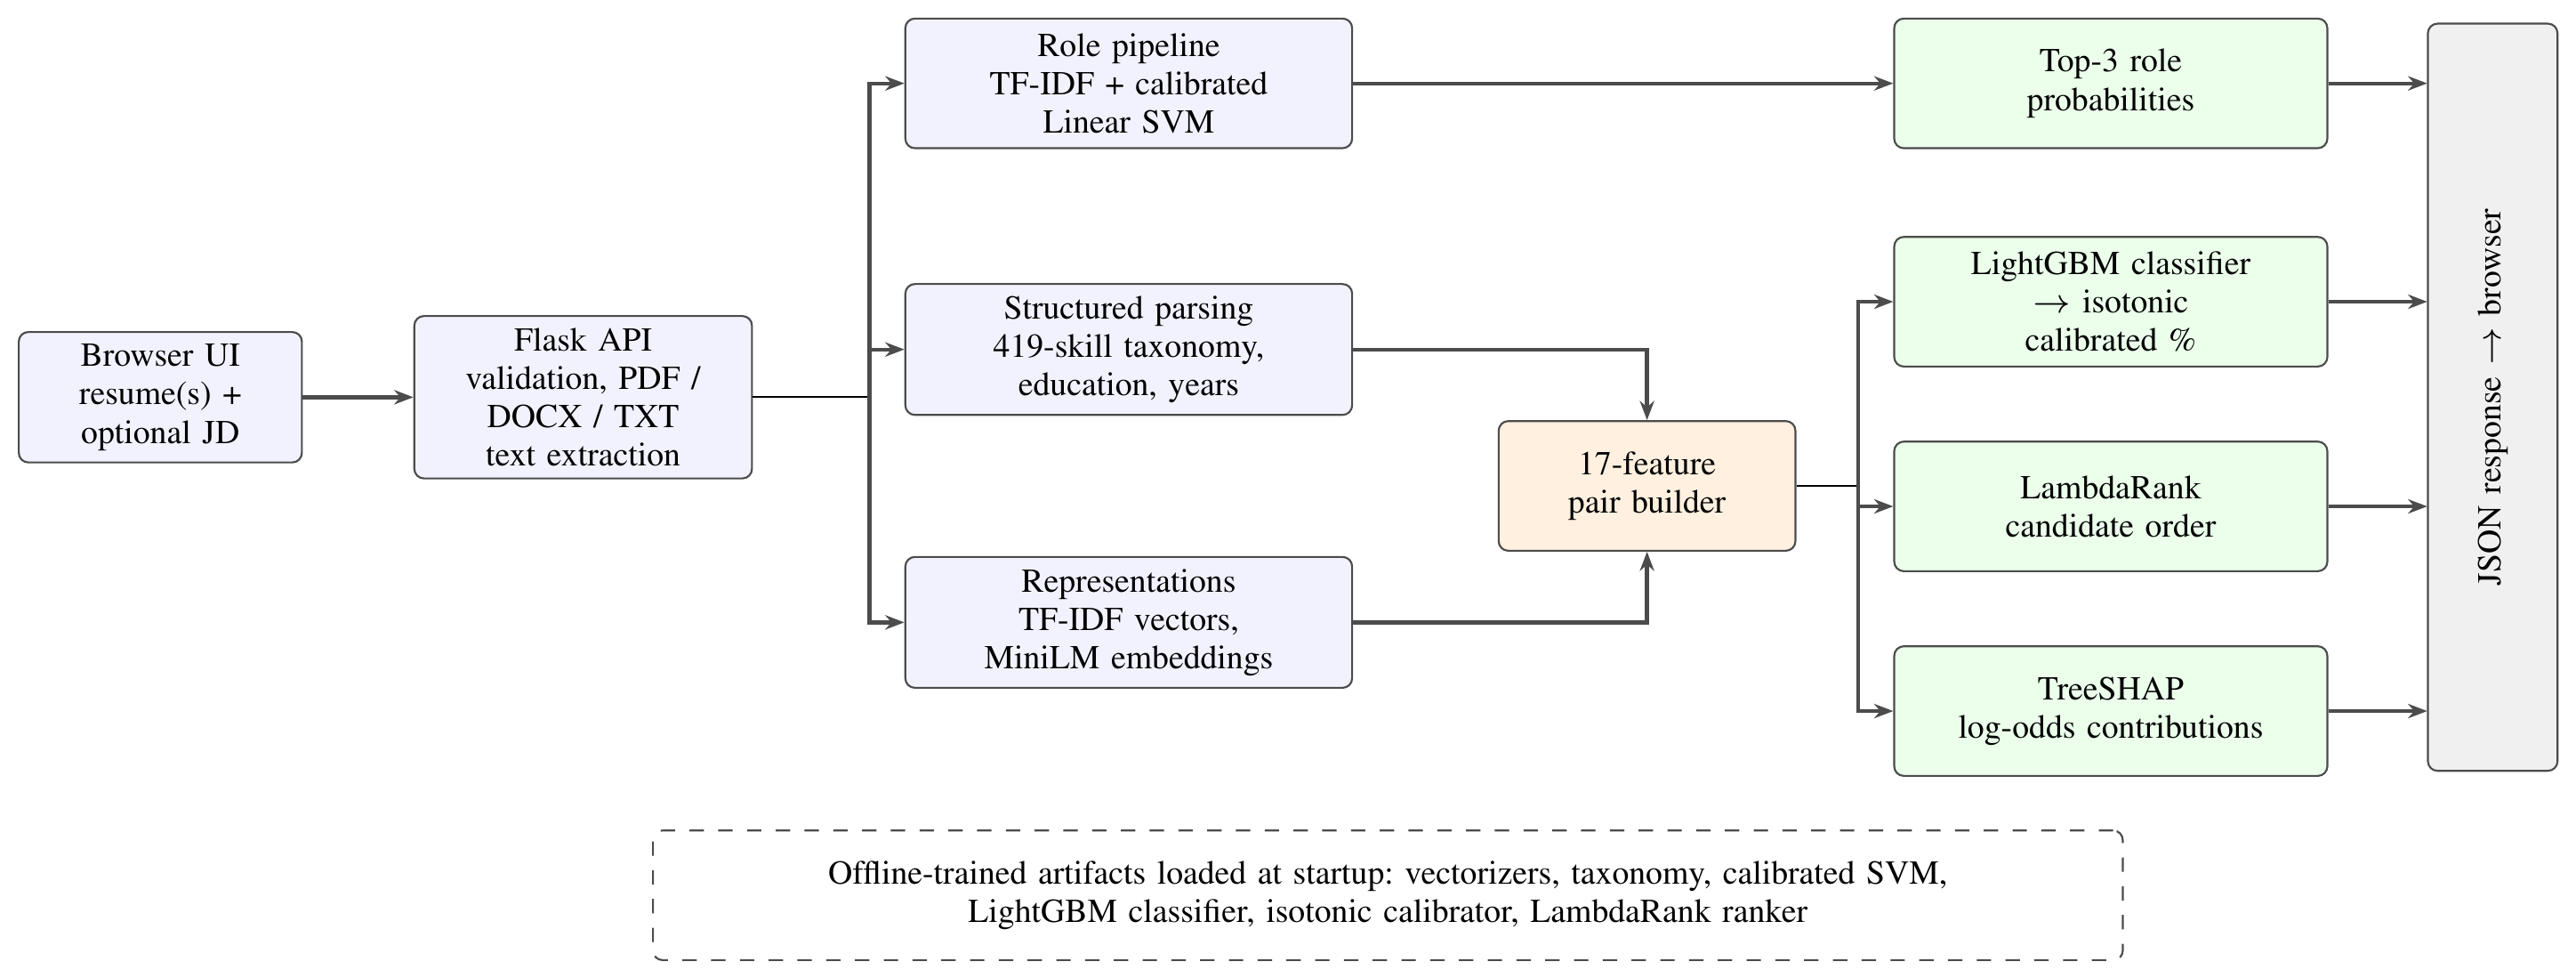
\includegraphics[width=0.92\textwidth]{figs/fig2.png}
\caption{Implemented inference architecture. Ranking order and displayed compatibility follow separate paths, and the role classifier is independent of pair scoring. Dashed elements are produced offline and loaded once.}
\label{fig:arch}
\end{figure*}

The single-analysis endpoint returns profile attributes and the top three role probabilities. When a job description is supplied, it also returns compatibility, dimension bars, skill and keyword gaps and explanations. The ranking endpoint accepts 2 to 30 readable resumes for one job (Algorithm~3), and a separate endpoint exposes the saved evaluation metrics. The interface assigns descriptive bands at 70, 45 and 25 percent; these are display rules, not validated hiring cutoffs.

\section{Experimental Setup}
\subsection{Implementation}
The system is written in Python with Flask, scikit-learn, LightGBM, Sentence-Transformers, NumPy, SciPy, pandas, joblib, pypdf and python-docx, plus an HTML/CSS/JavaScript interface. Source code and saved evaluation artifacts are available in the project repository \cite{b17}. Results are taken from the metric artifacts recorded during training (metrics.json and experiment\_report.json) and from the project report \cite{b18}. No training hardware specification, dependency lockfile, elapsed-time log or throughput benchmark was recorded, and the experiments were not repeated over multiple random seeds.

\subsection{Baselines and Metrics}
The matching baselines are skill coverage (keyword overlap), TF-IDF cosine and embedding cosine, together with a standardized Logistic Regression on the same 17 features. Role prediction is evaluated with accuracy, macro-F1 and per-class scores. Compatibility discrimination uses the area under the receiver operating characteristic curve (ROC-AUC) and average precision (AP; stored as ``PR-AUC'' in the project report). Probability quality is judged by the Brier score and the ten-bin ECE,
\begin{equation}
\mathrm{ECE}=\sum_{m=1}^{10}\frac{|B_m|}{N}\left|\mathrm{acc}(B_m)-\mathrm{conf}(B_m)\right|,
\end{equation}
\begin{equation}
\mathrm{Brier}=\frac{1}{N}\sum_{i=1}^{N}(\hat{p}_i-y_i)^2.
\end{equation}
Ranking uses exponential-gain discounted cumulative gain (DCG) normalized by the ideal ordering and averaged across jobs,
\begin{equation}
\mathrm{DCG@}k=\sum_{i=1}^{k}\frac{2^{\mathrm{rel}_i}-1}{\log_2(i+1)},\quad
\mathrm{NDCG@}k=\frac{\mathrm{DCG@}k}{\mathrm{IDCG@}k}
\end{equation}
Recall@10 and Precision@5 treat grades two and three as relevant.

\subsection{Protocols}
The ablation retrains an uncalibrated classifier and a ranker after removing each feature group, so its ROC-AUC and NDCG values originate from different estimators. Error analysis thresholds calibrated probabilities at 0.5. The identity-sensitivity probe prefixes names, pronouns or birth-year text to 120 sampled test-pair inputs; sampling is over pairs, so 120 distinct people are not guaranteed. In addition, 23 source-level utility, feature and request-validation checks were run on the application code without loading trained models. Twenty-two passed, and a DOCX file whose text sat only inside a table returned empty text. These checks demonstrate implementation behaviour, not trained-model accuracy.

\section{Results and Discussion}
\subsection{Occupational Classification}
The selected calibrated linear SVM reaches 71.43\% test accuracy and a macro-F1 of 0.6716 on 497 resumes. Its tuned cross-validation macro-F1 is 0.6277, against 0.6123 for tuned Logistic Regression and 0.6222 for the untuned Random Forest; Naive Bayes and KNN reach 0.4765 and 0.4899. Performance differs widely across classes (Fig.~\ref{fig:perclass}). Designer attains an F1 of 0.909, Information Technology 0.889 and HR 0.875, whereas BPO scores zero on four test records and Apparel reaches 0.333 on nineteen. The overall result shows useful category discrimination, but the small and difficult classes make a single accuracy figure inadequate for all categories.

\begin{figure}[!t]
\centering
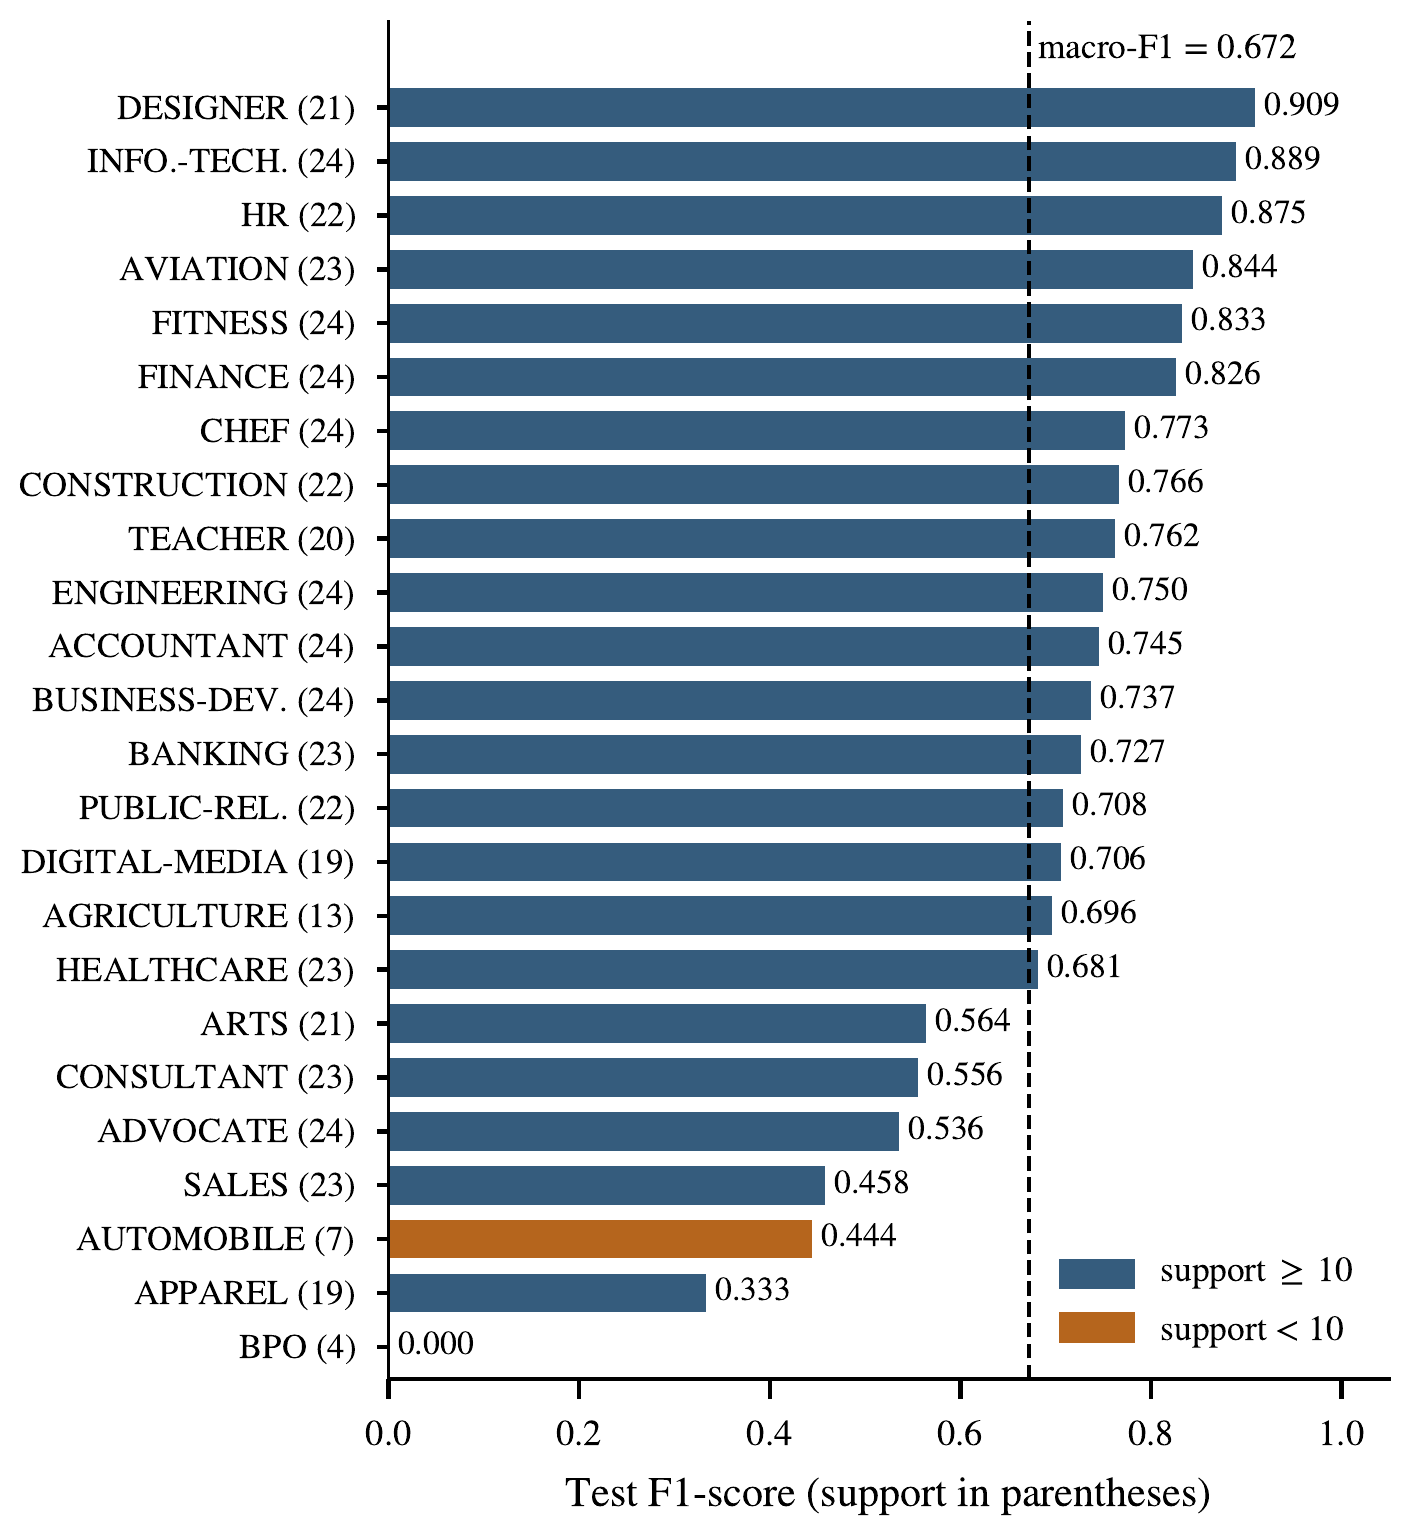
\includegraphics[width=0.88\columnwidth]{figs/fig3.png}
\caption{Per-class test F1 of the calibrated linear SVM (497 resumes), sorted by score. Orange marks classes with fewer than ten test records, whose estimates are unstable.}
\label{fig:perclass}
\end{figure}

\subsection{Compatibility and Ranking}
Table~\ref{tab:main} compares all recorded matching models. Logistic Regression has the highest ROC-AUC (0.8067), marginally above calibrated LightGBM (0.8041). Relative to TF-IDF cosine, calibrated LightGBM raises ROC-AUC by 0.0349 and NDCG@10 by 0.0567 in absolute terms. Combining features therefore improves discrimination on this benchmark, although the tree ensemble is not consistently better than the linear model. Because there is no repeated-seed experiment, confidence interval or significance test, these differences are descriptive only.

\begin{table}[!t]
\caption{Held-Out Weak-Label Benchmark Results (11,520 Pairs)}
\label{tab:main}
\centering
\footnotesize
\setlength{\tabcolsep}{2.2pt}
\resizebox{\columnwidth}{!}{%
\begin{tabular}{lcccccc}
\toprule
Model & ROC-AUC & AP & NDCG@5 & NDCG@10 & R@10 & P@5 \\
\midrule
Keyword overlap & 0.694 & 0.500 & 0.703 & 0.645 & 0.507 & 0.703 \\
TF-IDF cosine & 0.769 & 0.648 & 0.681 & 0.643 & 0.512 & 0.683 \\
Embedding cosine & 0.759 & 0.622 & 0.673 & 0.626 & 0.502 & 0.684 \\
Logistic Regression & 0.807 & 0.690 & 0.711 & 0.670 & 0.535 & 0.717 \\
LightGBM (raw) & 0.805 & 0.690 & 0.712 & 0.674 & 0.540 & 0.720 \\
LightGBM (calibrated) & 0.804 & 0.672 & 0.739 & 0.699 & 0.559 & 0.740 \\
LambdaRank (deployed) & 0.802 & 0.689 & 0.718 & 0.677 & 0.541 & 0.725 \\
\bottomrule
\end{tabular}}
\end{table}

Calibrated LightGBM records the highest NDCG@10 (0.6994), whereas the deployed LambdaRank ordering achieves 0.6770, and the two should not be conflated. The ranking gain of the calibrated classifier over its own raw scores also deserves scrutiny. Isotonic regression is non-decreasing, so it can merge distinct scores into ties but cannot reorder them. Candidate pools are assembled in relevance-correlated blocks (same category first, unrelated last) and evaluation uses a stable sort, so tied scores keep the favorable input order. NDCG@10 rises from 0.6738 to 0.6994 while ROC-AUC falls from 0.8052 to 0.8041, a pattern better explained by tie handling than by a superior ordering function. The similarity and overlap baselines can produce ties as well. The ranking results should be rerun with randomized candidate order or tie-aware expected metrics before any superiority is claimed.

\subsection{Calibration and Feature Contributions}
Isotonic calibration reduces LightGBM's ECE from 0.02331 to 0.01766, but the Brier score moves from 0.1545949 to 0.1546031, a negligible worsening (Table~\ref{tab:calib}). Logistic Regression has both a lower ECE (0.01152) and a lower Brier score (0.15386), so calibration does not make LightGBM the strongest probability estimator. Fig.~\ref{fig:diag}(a) shows mild overprediction in the high-score bins (a mean prediction of about 0.881 against an observed frequency of about 0.810 in the 0.8--0.9 bin). Calibration here describes the frequency of weak labels in this benchmark, not the probability of being hired.

\begin{table}[!t]
\caption{Probability Quality on Held-Out Pairs}
\label{tab:calib}
\centering
\small
\begin{tabular}{@{}lccc@{}}
\toprule
Model & Brier $\downarrow$ & ECE $\downarrow$ & ROC-AUC \\
\midrule
LightGBM (before isotonic) & 0.15459 & 0.02331 & 0.80524 \\
LightGBM (after isotonic) & 0.15460 & 0.01766 & 0.80406 \\
Logistic Regression & 0.15386 & 0.01152 & 0.8067 \\
\bottomrule
\end{tabular}
\end{table}

\begin{figure*}[!t]
\centering
\subfloat[Reliability by test bin]{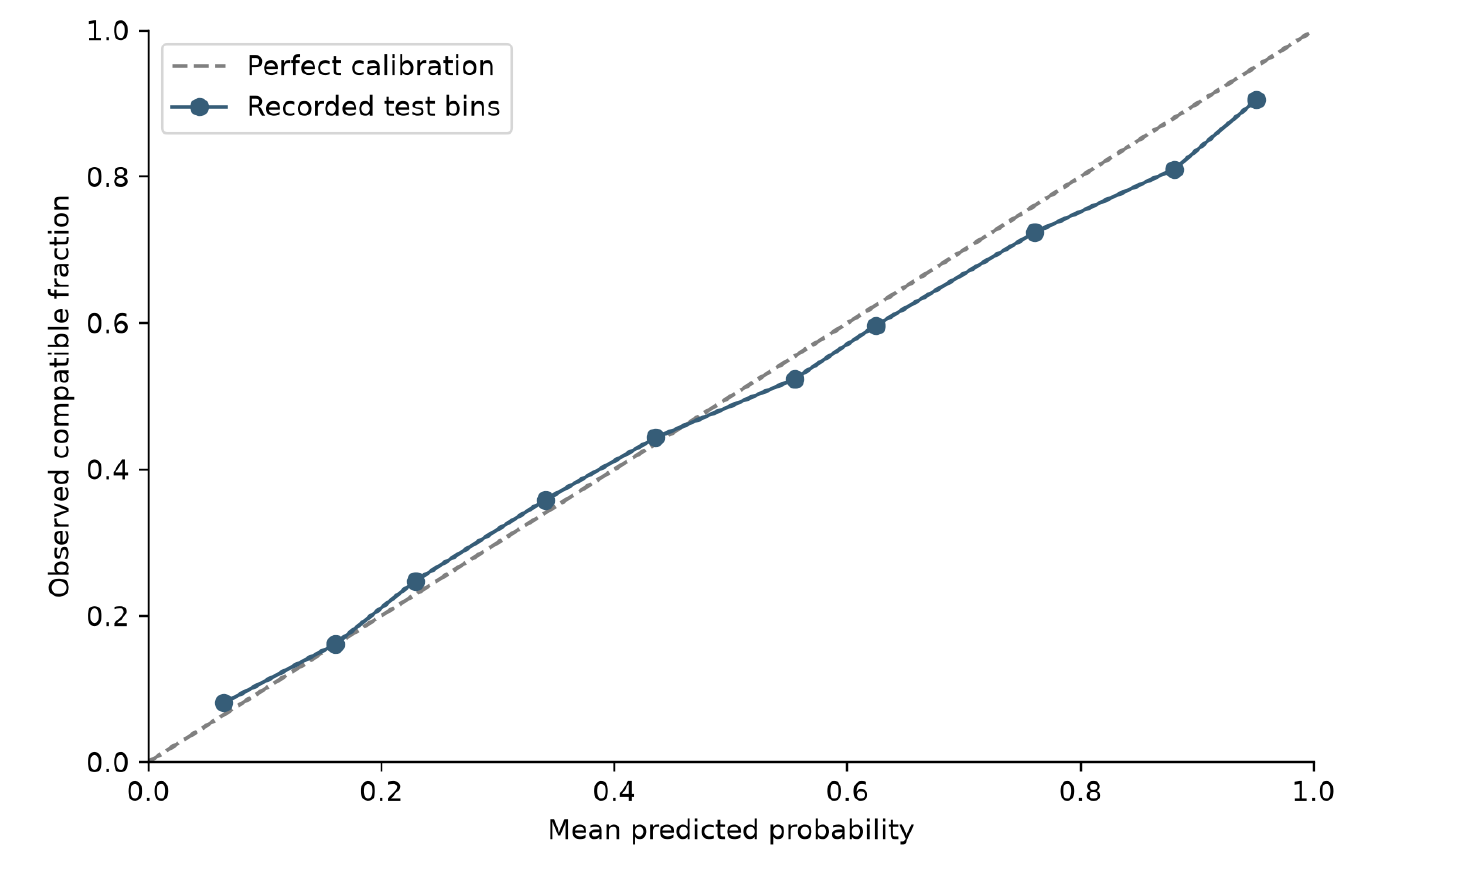
\includegraphics[width=0.46\textwidth]{figs/fig4a.png}\label{fig:diag_a}}
\hfill
\subfloat[Ten largest feature gains]{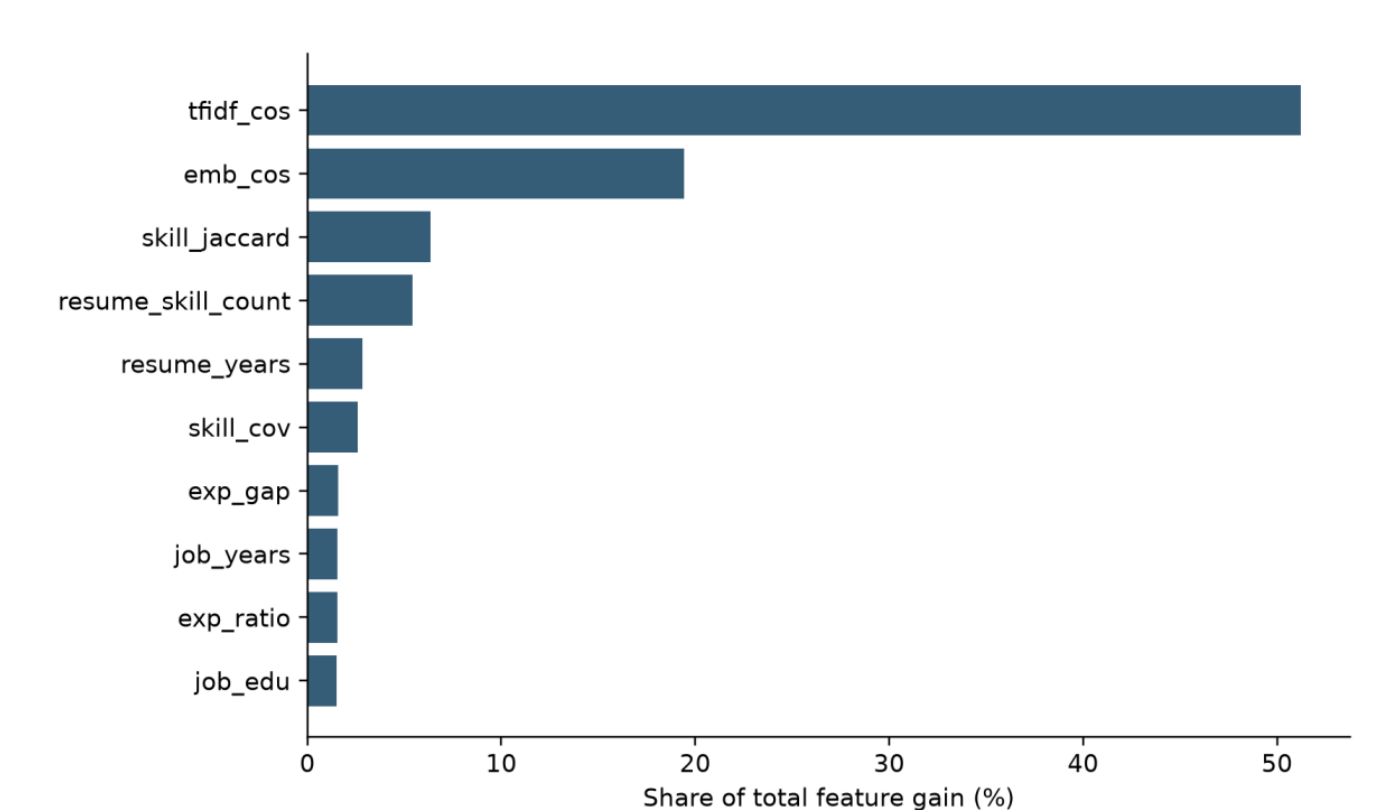
\includegraphics[width=0.46\textwidth]{figs/fig4b.png}\label{fig:diag_b}}
\caption{Recorded diagnostics of the calibrated compatibility model: (a) mean predicted probability against observed weak-label compatibility; (b) normalized feature gain. Gain is a model statistic, not a causal effect.}
\label{fig:diag}
\end{figure*}

Table~\ref{tab:ablation} shows that removing embeddings causes the largest fall in ablation ROC-AUC (0.8064 to 0.7789), removing TF-IDF lowers it to 0.7894 and removing skills to 0.7945. This supports the view that semantic, lexical and structured evidence complement one another. TF-IDF cosine accounts for 51.2\% of total feature gain and embedding cosine for 19.4\% (Fig.~\ref{fig:diag}(b)). Gain and ablation answer different questions, and correlated features can share importance unevenly. The small effects of experience and education agree with a label rule that does not depend on meeting those requirements, so they do not show that such qualifications are unimportant to employers.

\begin{table}[!t]
\caption{Feature-Group Ablation}
\label{tab:ablation}
\centering
\small
\begin{tabular}{@{}lccc@{}}
\toprule
Removed group & Clf.\ ROC-AUC & Clf.\ AP & Ranker NDCG@10 \\
\midrule
None (full) & 0.8064 & 0.6921 & 0.6770 \\
\midrule
Embedding & 0.7789 & 0.6522 & 0.6496 \\
TF-IDF & 0.7894 & 0.6583 & 0.6544 \\
Skills & 0.7945 & 0.6798 & 0.6640 \\
Experience & 0.8042 & 0.6887 & 0.6758 \\
Education & 0.8032 & 0.6914 & 0.6768 \\
\bottomrule
\end{tabular}
\end{table}

\subsection{Errors and Identity Sensitivity}
At a threshold of 0.5 the false-positive rate is 9.54\% and the false-negative rate is 50.44\%, so about half of the benchmark-positive pairs fall below the decision threshold. The most frequent false negatives are same-category pairs (Agriculture 94, Apparel 93, Consultant 84 and Healthcare 84 pairs). The most frequent false positives are Public Relations resumes against Arts jobs (14) and Information Technology resumes against BPO or Automobile jobs (13 and 12). The mean predicted probability rises from about 0.206 for grade zero (0.241 and 0.362 for grades one and two) to 0.552 for grade three. This indicates a graded association, but with considerable uncertainty even for same-category pairs. These findings do not support autonomous rejection at the default cutoff.

\begin{table}[!t]
\caption{Identity-Text Perturbations on 120 Test Pairs (Changes in Percentage Points)}
\label{tab:identity}
\centering
\small
\begin{tabular}{@{}lccc@{}}
\toprule
Variant & Mean $|\Delta p|$ & Max $|\Delta p|$ & Flips \\
\midrule
Female name & 1.03 & 13.00 & 2 \\
Male name & 0.96 & 15.62 & 1 \\
South-Asian name & 0.78 & 10.89 & 2 \\
East-Asian name & 0.54 & 10.66 & 1 \\
Older (born 1962) & 0.60 & 10.89 & 2 \\
\bottomrule
\end{tabular}
\end{table}

Table~\ref{tab:identity} converts the stored identity perturbations into percentage-point changes. Average effects are small, but the maximum reaches 15.62 points and every variant yields one or two threshold flips. No protected attribute is supplied as a separate engineered column, yet identity text can remain in the TF-IDF and embedding inputs or shift chunk boundaries. Because each variant bundles particular names and pronouns, the experiment cannot isolate demographic effects or establish group fairness; it is a sensitivity probe in the spirit of name-based audit studies \cite{b12}.

\subsection{Demonstration}
Fig.~\ref{fig:demo} shows the application on a Finance Analyst description. The finance resume receives a calibrated compatibility of 88\% with 57\% required-skill coverage (four of seven parsed job skills), and the predicted role is FINANCE at 80\% confidence. TF-IDF similarity contributes about $+1.767$ and embedding similarity $+0.631$ to the raw classifier log-odds, while the experience-related features contribute negatively despite full experience alignment. This reflects associations learned under weak labels and is not a normative finding that more experience lowers suitability. In the ranking view, an Accountant resume (98\%) is placed ahead of the Finance resume (88\%) and a Banking resume (40\%). The example shows how the system combines signals beyond a checklist; it illustrates behaviour and is not an accuracy experiment. The bars summarize measured features, the percentage is a calibrated proxy-label probability, and rank is a separate model output.

\begin{figure*}[!t]
\centering
\subfloat[Compatibility result and feature explanation]{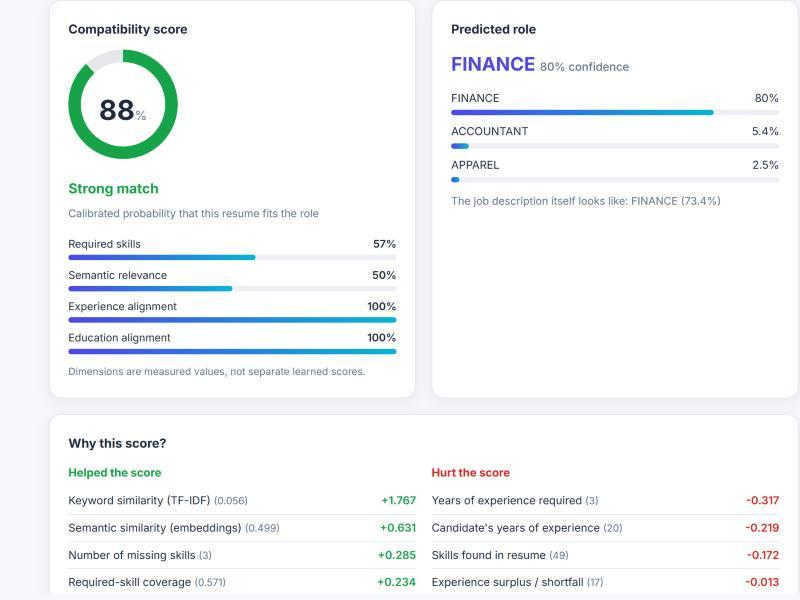
\includegraphics[width=0.40\textwidth]{figs/fig5a.png}\label{fig:demo_a}}
\hfill
\subfloat[Candidate ranking (top three rows)]{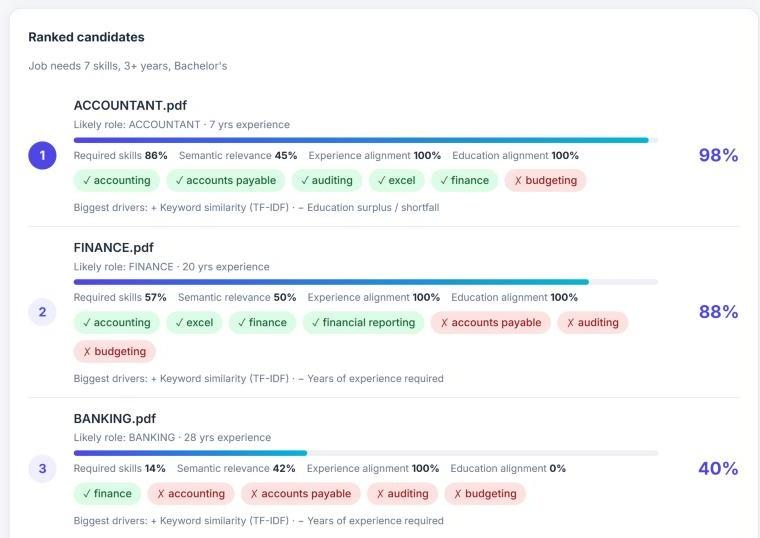
\includegraphics[width=0.46\textwidth]{figs/fig5b.png}\label{fig:demo_b}}
\caption{Application demonstration on a Finance Analyst job description (historical screenshots from the project, not a re-run of a newly trained model).}
\label{fig:demo}
\end{figure*}

\section{Limitations and Future Work}
The main limitation is construct validity. Synthetic descriptions and category relations approximate relevance without showing that real job requirements are met. Shared generation templates and incomplete skill-pool separation narrow what can be generalized, and record-level separation does not prove that no person appears on both sides. Calibration and model comparisons use different training allocations, and stable-sort tie effects, a single recorded split and the lack of uncertainty estimates restrict the comparative conclusions.

The extraction pipeline omits DOCX table content and image-only PDFs, applies approximate date and degree rules, and merges mandatory with preferred skills. Semantic truncation can discard later evidence, and experience estimates that depend on the current year, together with unpinned dependencies, hinder reproduction. The application has no measured load performance, formal user validation, or production privacy and access controls. No real hiring outcome, cost saving or fairness guarantee follows from the current results.

Future work should begin with authentic job advertisements, independently judged pair relevance, explicit annotation criteria and candidate-level separation. Randomized or tie-aware ranking evaluation, repeated splits and calibration checks under distribution shift would strengthen the evidence. Separate parsing of required and preferred skills, section-aware representations, optical character recognition (OCR) and table extraction would improve input fidelity, and domain-adapted encoders or cross-encoders should be compared against the existing lexical and linear baselines. Human review, correction of extracted profiles and population-level fairness analysis remain necessary before operational use.

\section{Conclusion}
This study combines structured extraction, lexical and semantic representations, calibrated compatibility, ranking and feature attribution in a single resume-analysis pipeline. The recorded experiments show 71.43\% role accuracy and better compatibility discrimination than any single similarity baseline, and the ablation supports complementary semantic and lexical signals. However, Logistic Regression remains competitive, isotonic calibration lowers ECE without improving the Brier score, and the ranking gains need to be reassessed with tie-aware evaluation. The high false-negative rate and the identity sensitivity underline the limits of category-derived supervision. The result is a research prototype whose behaviour on this benchmark can be inspected, and a starting point for validation on authentic resume--job relevance; it is not a validated hiring decision system.

\section*{Acknowledgment}
The authors thank their project guide, Dr.\ Gopinath M.\ P., for his guidance throughout this work.

\begin{thebibliography}{00}
\bibitem{b1} C. D. Manning, P. Raghavan, and H. Sch\"utze, \textit{Introduction to Information Retrieval}. Cambridge, U.K.: Cambridge Univ. Press, 2008. [Online]. Available: https://nlp.stanford.edu/IR-book/
\bibitem{b2} N. Reimers and I. Gurevych, ``Sentence-BERT: Sentence embeddings using Siamese BERT-networks,'' in \textit{Proc. Conf. Empirical Methods Natural Lang. Process. and 9th Int. Joint Conf. Natural Lang. Process. (EMNLP-IJCNLP)}, 2019, pp. 3982--3992.
\bibitem{b3} W. Wang, F. Wei, L. Dong, H. Bao, N. Yang, and M. Zhou, ``MiniLM: Deep self-attention distillation for task-agnostic compression of pre-trained transformers,'' in \textit{Proc. Adv. Neural Inf. Process. Syst. (NeurIPS)}, vol. 33, 2020, pp. 5776--5788.
\bibitem{b4} G. Ke \textit{et al.}, ``LightGBM: A highly efficient gradient boosting decision tree,'' in \textit{Proc. Adv. Neural Inf. Process. Syst.}, vol. 30, 2017, pp. 3146--3154.
\bibitem{b5} C. J. C. Burges, ``From RankNet to LambdaRank to LambdaMART: An overview,'' Microsoft Research, Redmond, WA, USA, Tech. Rep. MSR-TR-2010-82, 2010.
\bibitem{b6} K. J\"arvelin and J. Kek\"al\"ainen, ``Cumulated gain-based evaluation of IR techniques,'' \textit{ACM Trans. Inf. Syst.}, vol. 20, no. 4, pp. 422--446, 2002.
\bibitem{b7} S. M. Lundberg and S.-I. Lee, ``A unified approach to interpreting model predictions,'' in \textit{Proc. Adv. Neural Inf. Process. Syst.}, vol. 30, 2017, pp. 4765--4774.
\bibitem{b8} S. M. Lundberg \textit{et al.}, ``From local explanations to global understanding with explainable AI for trees,'' \textit{Nature Mach. Intell.}, vol. 2, no. 1, pp. 56--67, 2020.
\bibitem{b9} Scikit-learn developers, ``Probability calibration,'' scikit-learn User Guide. [Online]. Available: https://scikit-learn.org/stable/modules/calibration.html. Accessed: Oct. 26, 2026.
\bibitem{b10} C. Guo, G. Pleiss, Y. Sun, and K. Q. Weinberger, ``On calibration of modern neural networks,'' in \textit{Proc. Int. Conf. Mach. Learn. (ICML)}, PMLR, vol. 70, 2017, pp. 1321--1330.
\bibitem{b11} A. Ratner \textit{et al.}, ``Snorkel: Rapid training data creation with weak supervision,'' \textit{Proc. VLDB Endowment}, vol. 11, no. 3, pp. 269--282, 2017.
\bibitem{b12} M. Bertrand and S. Mullainathan, ``Are Emily and Greg more employable than Lakisha and Jamal? A field experiment on labor market discrimination,'' \textit{Amer. Econ. Rev.}, vol. 94, no. 4, pp. 991--1013, 2004.
\bibitem{b13} M. Raghavan, S. Barocas, J. Kleinberg, and K. Levy, ``Mitigating bias in algorithmic hiring: Evaluating claims and practices,'' in \textit{Proc. ACM Conf. Fairness, Accountability, Transparency (FAT*)}, 2020, pp. 469--481.
\bibitem{b14} S. Bhawal, ``Resume dataset,'' Kaggle. [Online]. Available: https://www.kaggle.com/datasets/snehaanbhawal/resume-dataset. Accessed: Oct. 26, 2026.
\bibitem{b15} Sentence-Transformers, ``all-MiniLM-L6-v2,'' Hugging Face model card. [Online]. Available: https://huggingface.co/sentence-transformers/all-MiniLM-L6-v2. Accessed: Oct. 26, 2026.
\bibitem{b16} F. Pedregosa \textit{et al.}, ``Scikit-learn: Machine learning in Python,'' \textit{J. Mach. Learn. Res.}, vol. 12, pp. 2825--2830, 2011.
\bibitem{b17} Kiwi-Supreme, ``Resume Analyser,'' GitHub repository with source code and saved evaluation artifacts (models/metrics.json, models/experiment\_report.json). [Online]. Available: https://github.com/Kiwi-Supreme/Resume-Analyser. Accessed: Oct. 26, 2026.
\bibitem{b18} S. Srivastava and M. Subash, ``Resume analysis and job compatibility prediction using machine learning,'' unpublished project report, Vellore Inst. Technol., Vellore, India, 2026.
\end{thebibliography}

\end{document}
